\documentclass[unicode, 12pt, a4paper,oneside]{article}
\usepackage{booktabs}
\usepackage[utf8]{inputenc}
\usepackage[russian]{babel}
\usepackage{amsmath}
\usepackage{graphicx}
\usepackage{float}
\begin{document}
    \title{Лабораторная работа №1\\Ларионов Даниил\\НФИбд-01-16\\Вариант 6}
    \maketitle
    \section{Модель}
    В общем случае модель боевых действий между двумя сторонами определяется эффективность боевых подразделений, скоростью подхода подкреплений и различными небоевыми факторами, влияющими на убыль личного состава. Модель задается следующей системой ДУ: 
    $$
    \begin{cases}
    \frac{dx}{dt} = -ax(t) - by(t) + P(t) \\
    \frac{dy}{dt} = -cx(t) - hy(t) + Q(t)
    \end{cases}
    $$
    Где x(t), y(t) - функция численности армии x и y соотв. от времени. a, h - коэффициент влияния сторонних факторов, b,c - коэффициент эффективности боевых действий с обеих сторон. Так же задаются начальные условия в виде $x_0, y_0$ - начальных численностей армий.
    \subsection{Боевые действия с партизанскими отрядами}
    В случае использования стороной y партизанских отрядов скорость убыли численности её личного состава в результате действий противника так же зависит от непосредственно численности личного состава армии y в момент t. Иными словами:
    $$
    \begin{cases}
    \frac{dx}{dt} = -ax(t) - by(t) + P(t) \\
    \frac{dy}{dt} = -cx(t)y(t) - hy(t) + Q(t)
    \end{cases}
    $$
    
    \section{Задача}
    Даны следующие модели боевых действий:
    \begin{itemize}
        \item Боевые действия между регулярными армиями X, Y:
        $$
        \begin{cases}
        \frac{dx}{dt} = -0.34x(t) - 0.72y(t) + sin(t + 10) \\
        \frac{dy}{dt} = -0.89x(t) - 0.43y(t) + cos(t + 20)
        \end{cases}
        $$
        \item Боевые действия между регулярными армиями c применением партизанских отрядов X, Y:
        $$
        \begin{cases}
        \frac{dx}{dt} = -0.12x(t) - 0.51y(t) + sin(20t) \\
        \frac{dy}{dt} = -0.3x(t)y(t) - 0.61y(t) + cos(13t)
        \end{cases}
        $$
    \end{itemize}
    Начальные условия для моделей одинаковы: численность армии x = 50000, y = 69000.
    
    \section{Результаты}
    \subsection{График для первой моедли (Регулярные армии)}
    \begin{figure}[H]
        \centering
        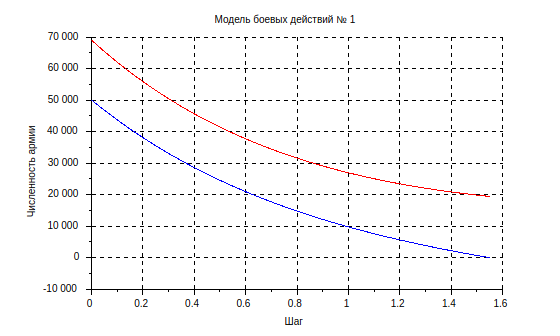
\includegraphics{lab02/lab2-graph0.png}
        \caption{График числа солдат в каждой армии от времени}
        \label{fig:model1}
    \end{figure}
    В данном случае проиграла армия X. Численность солдат в ней достигла нуля в момент времени t=1.55.
    \subsection{График для второй модели (Регулярные армии + партизаны)}
    \begin{figure}[H]
        \centering
        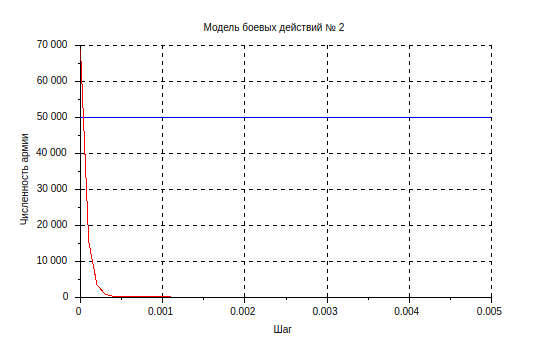
\includegraphics{lab02/lab2-graph.png}
        \caption{График числа солдат от времени}
        \label{fig:model2l}
    \end{figure}
    В данном случае, скорее всего имеет место ошибка в расчетах или в составлении системы ДУ, посколько Армия Y полностью вымирает в момент времени t=0.0004.
    
    
\end{document}